\chapter{Начало работы с инструкцией SELECT}
\section{Использование FROM и SELECT}

% \noindent Функция возвращения книги в библиотеку:
\begin{lstlisting}[label=lst:funcReturn, caption=Пример работы, language=sql]
	SELECT empid, firstname + N' ' + lastname AS fullname
	FROM HR.Employees; 
\end{lstlisting}

Дубликаты возможны в результате запроса и вы хотите их удалить, чтобы получить на выходе
реляционный результат, этого можно добиться, добавив предложение DISTINCT, как
показано в следующем примере: 

\begin{lstlisting}[label=lst:funcReturn, caption=Пример работы DISTINCT, language=sql]
	SELECT DISTINCT country, region, city
	FROM HR.Employees; 
\end{lstlisting}


Существует интересное различие между стандартным языком SQL и T-SQL с точки
зрения минимальных требований запроса SELECT. В соответствии со стандартным
языком SQL, запрос должен иметь как минимум предложения FROM и SELECT. Напротив, T-SQL поддерживает запрос SELECT, содержащий только предложение SELECT
без предложения FROM. 


\begin{lstlisting}[label=lst:funcReturn, language=sql]
	SELECT 10 AS col1, 'ABC' AS col2; 
\end{lstlisting}	


\begin{figure}[h!]
	\begin{center}
		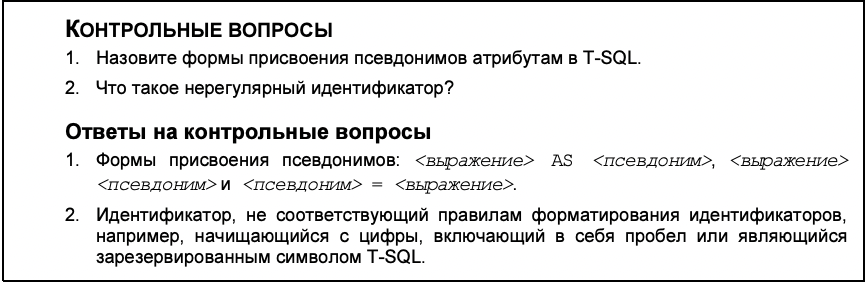
\includegraphics[width=0.8\textwidth]{img/control6.png}
	\end{center}
	\captionsetup{justification=centering}
\end{figure}


\subsection*{Резюме занятия}
\begin{itemize}
	\item Предложение FROM — это первое предложение, которое логически обрабатывается в запросе SELECT. В этом предложении указываются таблицы, к которым адресован запрос, и табличные операторы. В предложении FROM можно присваивать таблицам псевдонимы с именами по своему выбору и затем использовать псевдоним таблицы в качестве префикса к именам атрибутов. 
	\item С помощью предложения SELECT можно указать выражения, определяющие результирующие атрибуты. Можно присваивать результирующим атрибутам собственные псевдонимы и таким образом получать реляционный результат. Если в результате запроса возможно получение дубликатов, их следует удалить с помощью предложения DISTINCT.
	\item При использовании регулярных идентификаторов в качестве имен объектов или атрибутов применение разделителей является необязательным. Если используются нерегулярные идентификаторы, разделители обязательны. 
\end{itemize}

\subsection*{Закрепление материала}

\begin{figure}[h!]
	\begin{center}
		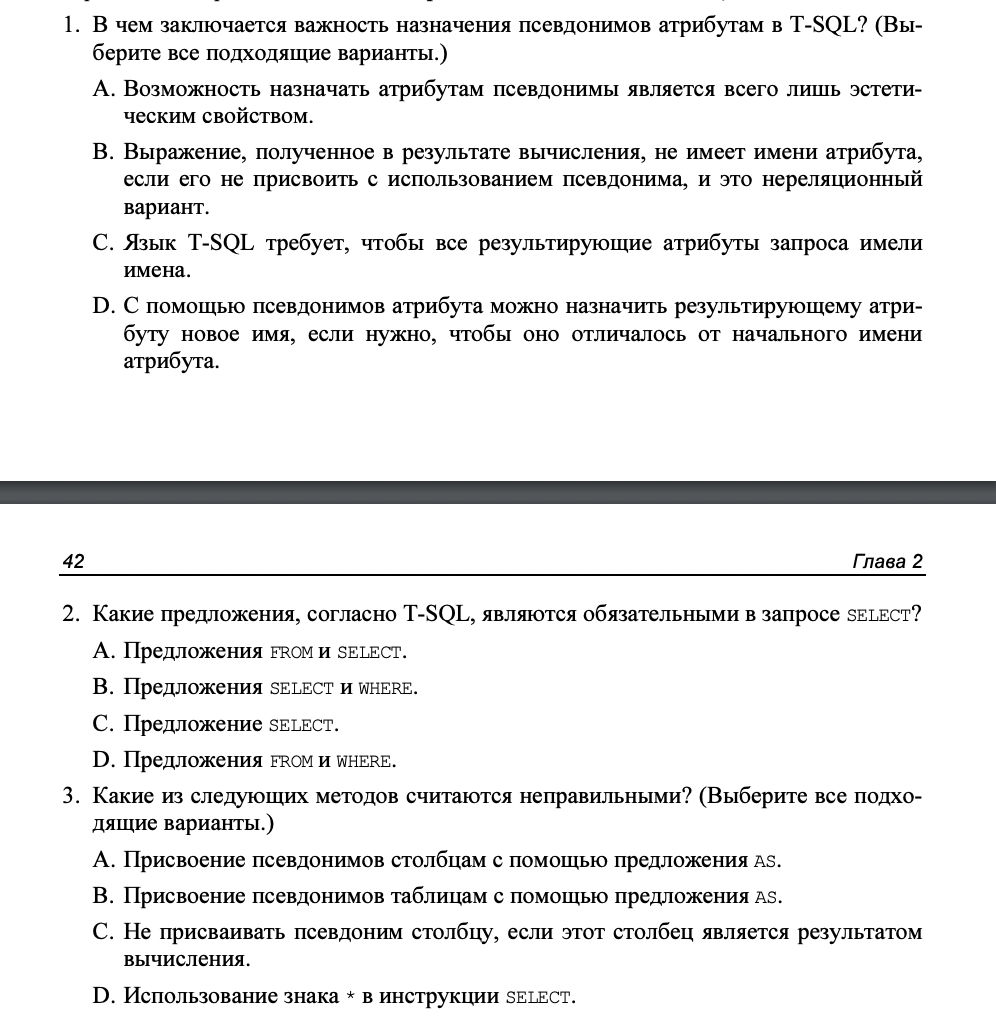
\includegraphics[width=0.9\textwidth]{img/zakrep3.png}
	\end{center}
	\captionsetup{justification=centering}
\end{figure}
\newpage

\subsection*{Ответы}

\begin{figure}[h!]
	\begin{center}
		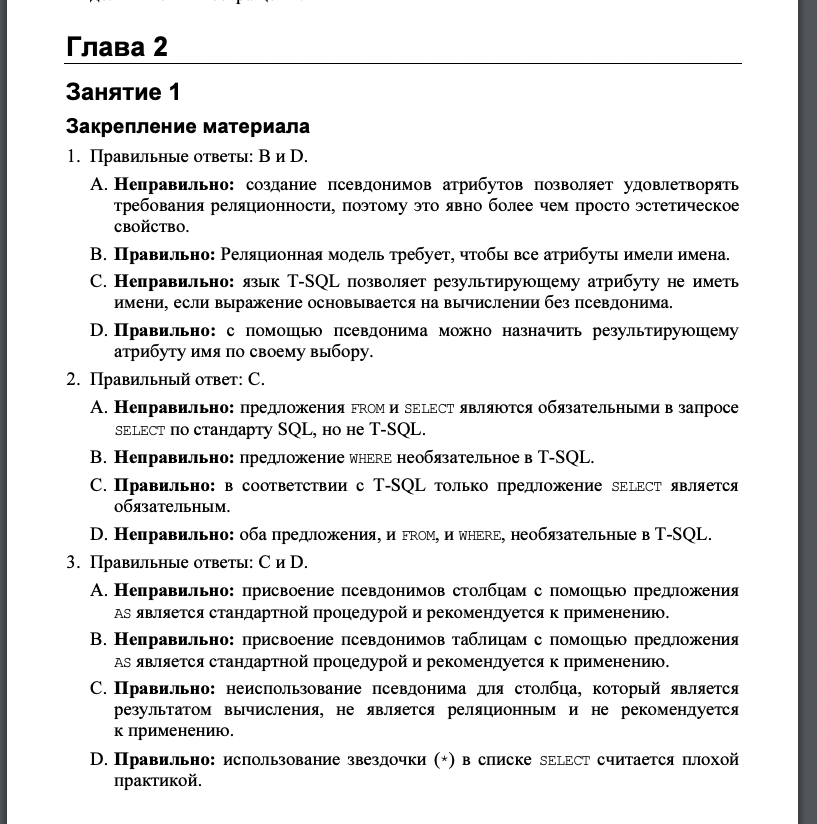
\includegraphics[width=0.9\textwidth]{img/ans3.png}
	\end{center}
	\captionsetup{justification=centering}
\end{figure}
\newpage




\section{Работа с типами данных и встроенными функциями}

Подробную информацию и технические подробности о типах данных можно найти в электронной документации по SQL Server 2012 в разделе <<Типы данных (Transact-SQL)>> по адресу Начало работы с инструкцией SELECT
\url{http://msdn.microsoft.com/ru-ru/library/ms187752(v=SQL.110).aspx}. Для получения дополнительных сведений о встроенных функциях см. раздел <<Встроенные функции (Transact-SQL)>> по адресу \url{http://msdn.microsoft.com/ru-ru/library/ms174318(v=SQL.110).aspx}. 

Данные с плавающей точкой являются приближенными; поэтому не все значения в диапазоне такого типа данных могут быть представлены точно. (Эти сведения можно найти в электронной документации для SQL Server 2012 в статье
<<Типы данных float and real Transact-SQL>> по адресу \url{http://msdn.microsoft.com/ruru/library/ms173773.aspx}.

При использовании символьных строк возникает вопрос о выборе обычных типов
символьных данных (CHAR, VARCHAR) или типов в кодировке Unicode (NCHAR,
NVARCHAR). Первый тип данных использует 1 байт памяти на символ и поддерживает
только один язык (на основании параметров сортировки), кроме английского. Последний тип данных использует 2 байта памяти на символ (без сжатия) и поддерживает несколько языков.

Литералы символьных строк в кодировке Unicode разделяются с помощью заглавной буквы N и затем одиночных кавычек, как в случае N'abc'.

<<Приоритет типов данных (Transact-SQL)>> на странице \url{http://msdn.microsoft.com/ru-ru/library/ms190309.aspx}.

\subsection{Выбор типов данных для ключей}
Для генерации суррогатных ключей, как правило, используются следующие элементы:

\begin{itemize}
	\item \textbf{Свойство столбца идентификаторов.} Свойство, которое автоматически генерирует ключи в атрибуте числового типа с масштабом 0; т. е. любого целочисленного типа (TINYINT, SMALLINT, INT, BIGINT) или типа NUMERIC/DECIMAL с масштабом 0.  
	\item \textbf{Объект последовательности.} Независимый объект в базе данных, из которого можно получить новые объекты последовательности. Так же как и свойство столбца идентификаторов, он поддерживает любой числовой тип данных с масштабом 0. В отличие от него, он не привязан к конкретному столбцу; напротив, как уже было сказано, это независимый объект в базе данных. Также можно запросить новое значение объекта последовательности перед его использованием.
	\item \textbf{Непоследовательные GUID.} Можно генерировать непоследовательные глобальные уникальные идентификаторы для их сохранения в атрибуте типа UNIQUEIDENTIFIER. Для генерации нового GUID вы можете использовать функцию T-SQL NEWID, вызывая его, например, с выражением по умолчанию, прикрепленным к столбцу. Его также можно генерировать где угодно — например, на клиенте, — с помощью программного интерфейса (API), который генерирует новый GUID. Уникальность идентификаторов GUID гарантирована в пространстве и времени.
	\item \textbf{Последовательные GUID.} Можно генерировать последовательные идентификаторы GUID с помощью функции T-SQL NEWSEQUENTIALID. 
	\item \textbf{Пользовательские решения.} Если вы не хотите использовать для генерации ключей встроенные инструменты, предлагаемые SQL Server, следует разработать собственное пользовательское решение. В таком случае тип данных для ключа зависит от пользовательского решения. 
\end{itemize}

\begin{figure}[h!]
	\begin{center}
		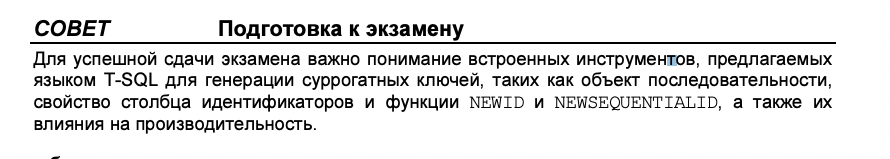
\includegraphics[width=0.9\textwidth]{img/advice1.png}
	\end{center}
	\captionsetup{justification=centering}
\end{figure}

Обратите внимание, если вы решили остановиться на последовательных ключах и к тому же числового типа, можно всегда начинать с наименьших значений выбранного типа данных, чтобы использовать весь диапазон. Например, для типа INT нужно начинать не с 1, а с числа –2 147 483 648. 

Полный список функций, а также технические детали и элементы синтаксиса приведены в электронной документации для SQL Server 2012 в разделе <<Типы данных и функции даты и времени (Transact-SQL)>> по адресу \url{http://msdn.microsoft.com/ru-ru/library/ms186724(v=SQL.110).aspx}.

С помощью функции FORMAT можно форматировать входное значение на основе строки форматирования и дополнительно указать культуру (язык и региональные параметры) в качестве третьего входного параметра там, где это имеет смысл. \url{http://msdn.microsoft.com/ru-ru/library/hh213505(v=sql.110).aspx}.

\subsection{Выражение CASE и связанные с ним функции}

\begin{lstlisting}[label=lst:funcReturn, caption=Пример работы CASE, language=sql]
	SELECT productid, productname, unitprice, discontinued,
	CASE discontinued
	WHEN 0 THEN 'No'
	WHEN 1 THEN 'Yes'
	ELSE 'Unknown'
	END AS discontinued_desc
	FROM Production.Products; 
\end{lstlisting}


\subsection{Функция COALESCE}


Функция COALESCE принимает список выражений на вход и возвращает первое выражение, не равное NULL, или NULL, если все выражения имеют значение NULL. Например, функция COALESCE(NULL, 'x', 'y') возвращает 'x'. В более общем смысле,
функция

\begin{lstlisting}[label=lst:funcReturn, language=sql]
	COALESCE(<exp1>, <exp2>, ..., <expn>); 
\end{lstlisting}
аналогична
\begin{lstlisting}[label=lst:funcReturn, language=sql]
CASE
	WHEN <exp1> IS NOT NULL THEN <exp1>
	WHEN <exp2> IS NOT NULL THEN <exp2>
	...
	WHEN <expn> IS NOT NULL THEN <exp2>
	ELSE NULL
END
\end{lstlisting}
Типичным использованием функции COALESCE является замена значения NULL чемлибо другим. Например, функция COALESCE(region, '') возвращает значение региона, если это не NULL, и пустую строку, если это NULL. 

\begin{figure}[h!]
	\begin{center}
		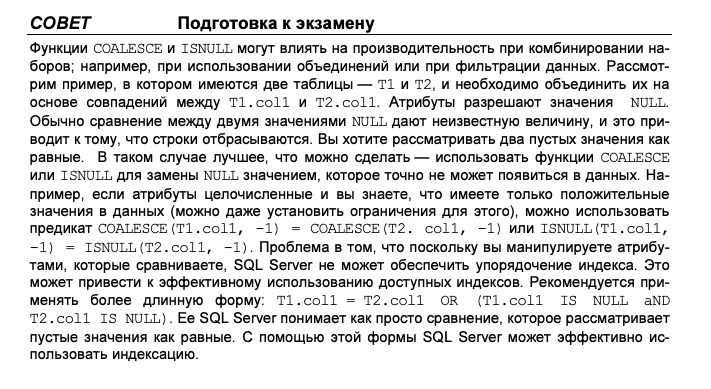
\includegraphics[width=1\textwidth]{img/advice2.png}
	\end{center}
	\captionsetup{justification=centering}
\end{figure}

\begin{figure}[h!]
	\begin{center}
		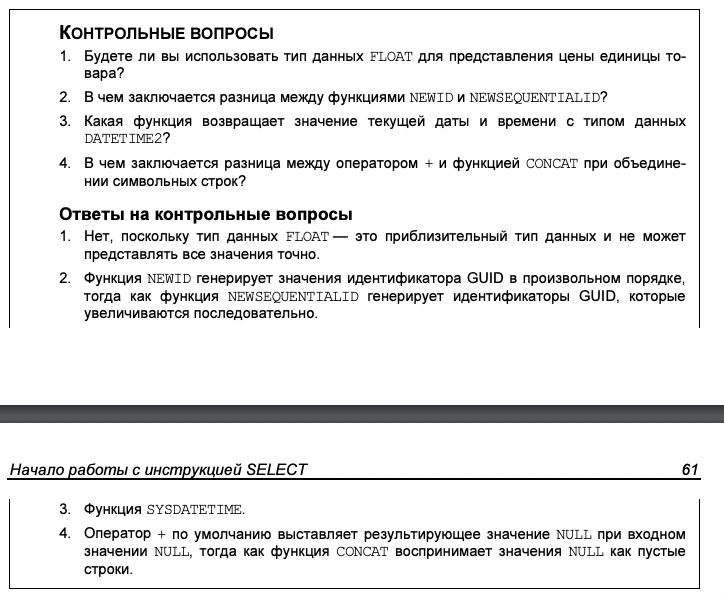
\includegraphics[width=0.9\textwidth]{img/control7.png}
	\end{center}
	\captionsetup{justification=centering}
\end{figure}

\newpage
\subsection*{Практикум}

\begin{figure}[h!]
	\begin{center}
		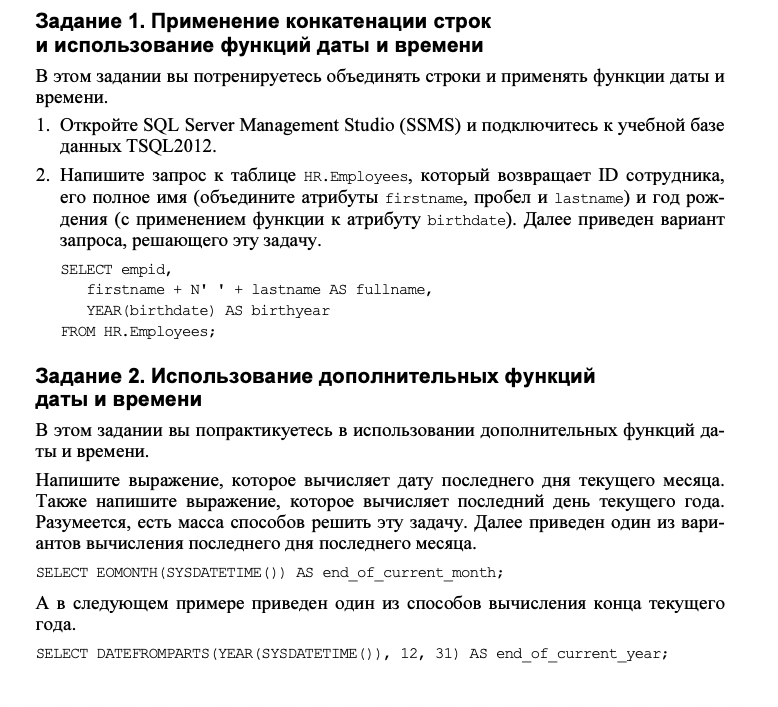
\includegraphics[width=1\textwidth]{img/prac1.png}
	\end{center}
	\captionsetup{justification=centering}
\end{figure}
\clearpage

\begin{figure}[h!]
	\begin{center}
		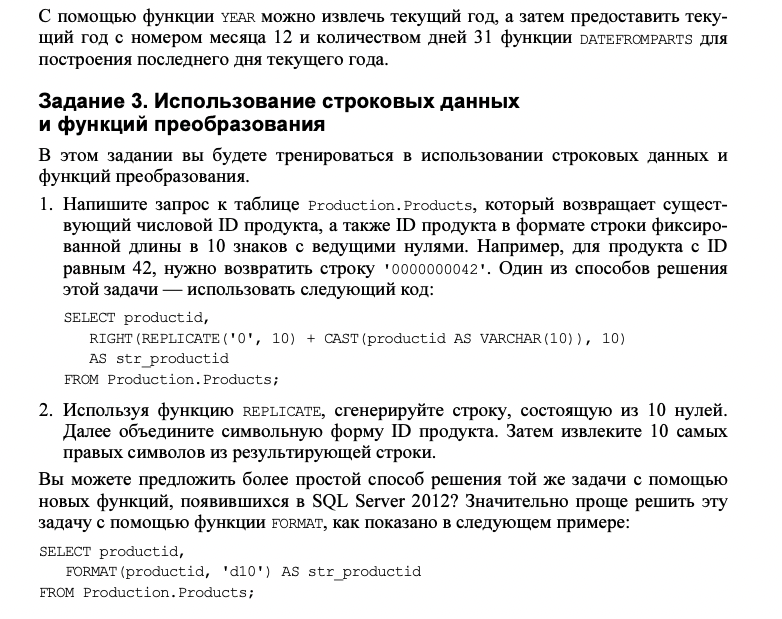
\includegraphics[width=0.9\textwidth]{img/prac2.png}
	\end{center}
	\captionsetup{justification=centering}
\end{figure}


\subsection*{Резюме занятия}
\begin{itemize}
	\item Выбор типа данных для атрибутов оказывает исключительно важное влияние на
	функциональность и производительность кода T-SQL, взаимодействующего
	с данными — и еще в большей степени это справедливо для атрибутов, используемых в ключах. Поэтому выбору типов данных следует уделять очень большое внимание.
	\item Язык T-SQL поддерживает множество функций, которые можно использовать
	для манипулирования данными даты и времени, символьными строковыми данными и другими типами данных. Помните, что язык T-SQL в основном был
	предназначен для обработки данных, а не для форматирования или подобных
	задач. Таким образом, в этих областях, как правило, можно получить только
	базовую поддержку. Подобные задачи, как правило, лучше всего выполнять на
	клиенте. 
	\item Язык T-SQL предоставляет выражение CASE, которое позволяет возвращать значение с использованием условной логики, а также множество функций, которые можно рассматривать сокращенными вариантами выражения CASE. 
\end{itemize}


\subsection*{Закрепление материала}

\begin{figure}[h!]
	\begin{center}
		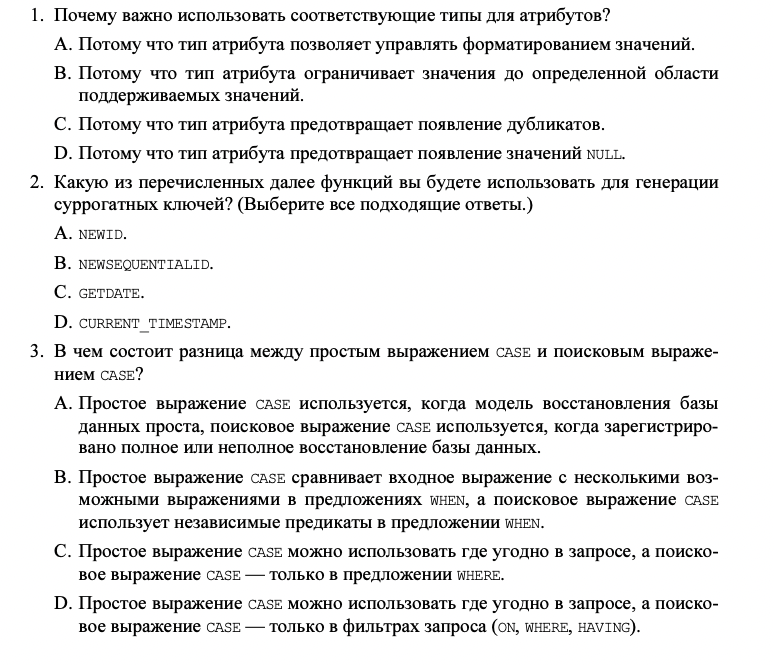
\includegraphics[width=0.9\textwidth]{img/zakrep4.png}
	\end{center}
	\captionsetup{justification=centering}
\end{figure}

\subsection*{Ответы}

\begin{figure}[h!]
	\begin{center}
		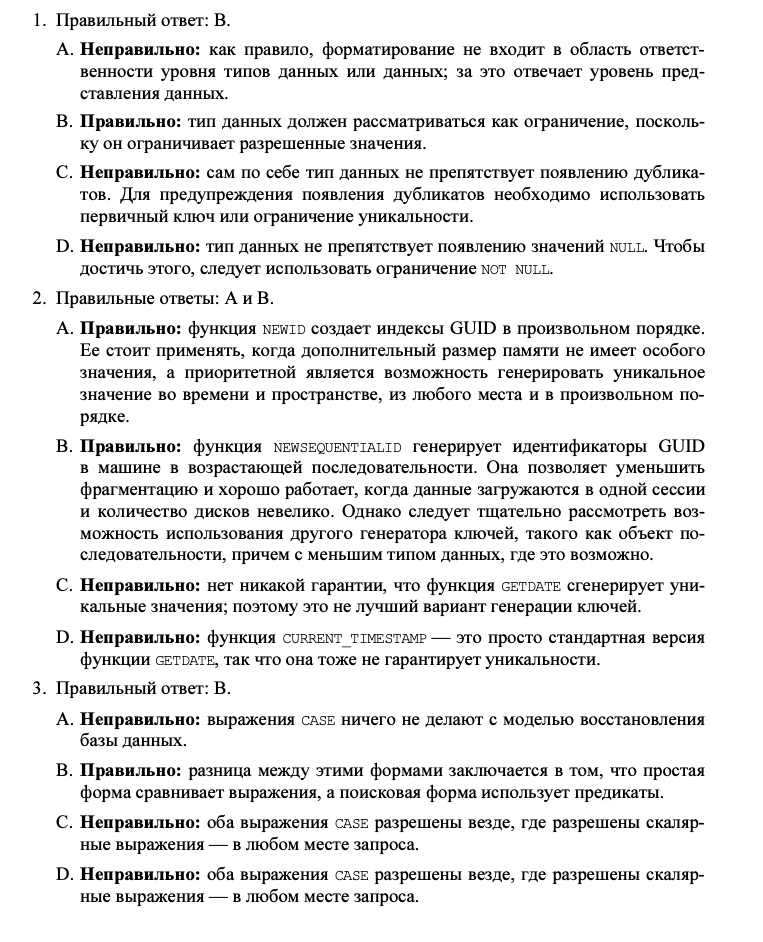
\includegraphics[width=0.7\textwidth]{img/ans4.png}
	\end{center}
	\captionsetup{justification=centering}
\end{figure}

\newpage
\subsection*{Упражнения}

\begin{figure}[h!]
	\begin{center}
		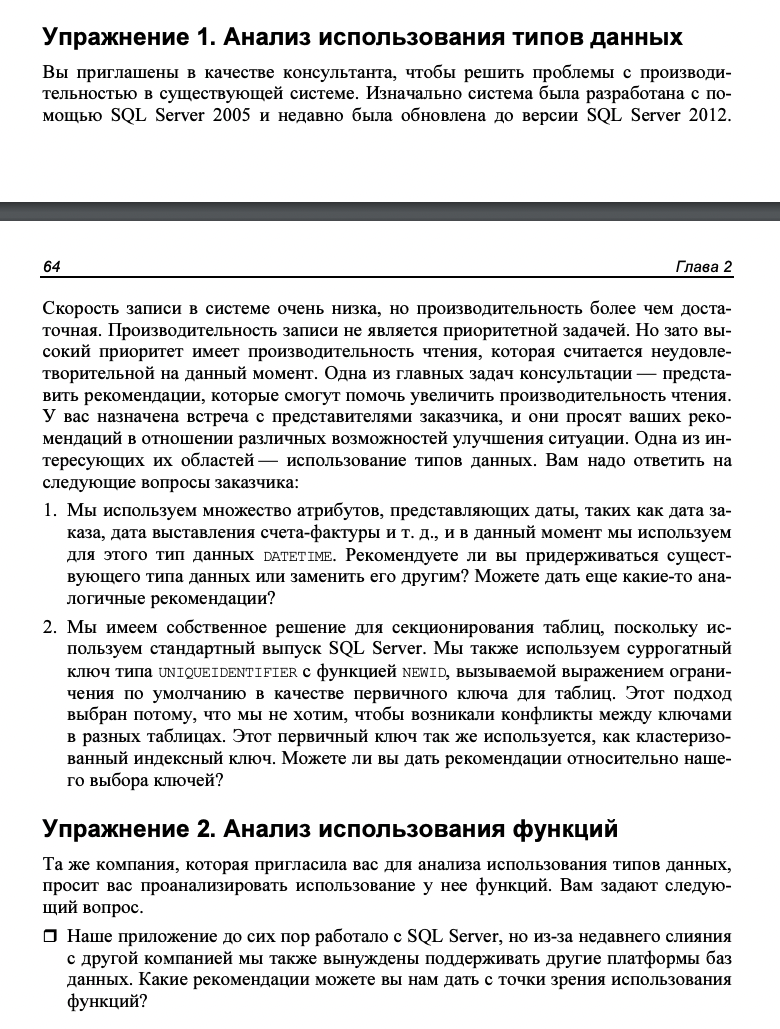
\includegraphics[width=0.9\textwidth]{img/ex2.png}
	\end{center}
	\captionsetup{justification=centering}
\end{figure}
\clearpage
\subsection*{Ответы}

\begin{figure}[h!]
	\begin{center}
		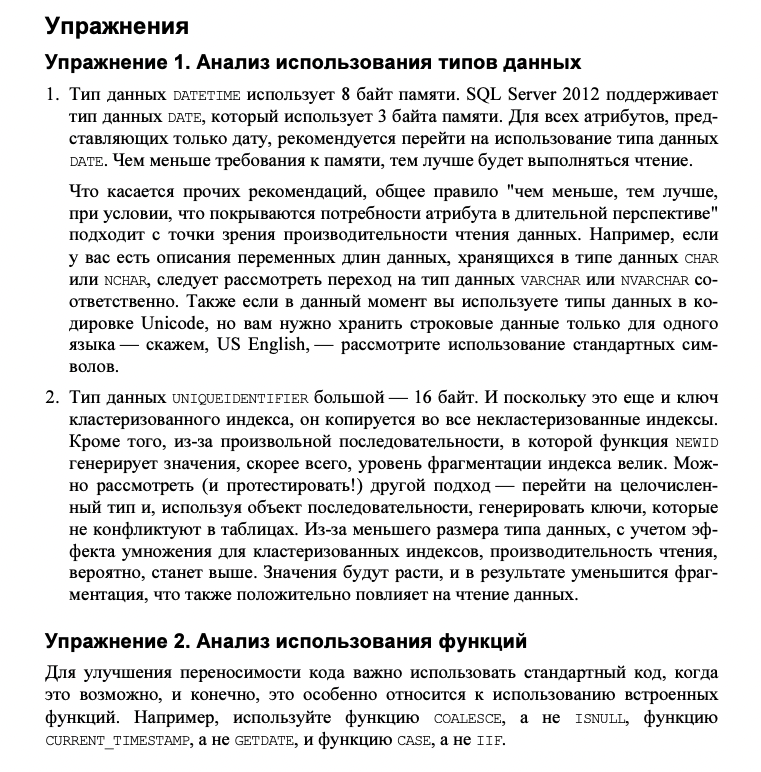
\includegraphics[width=0.9\textwidth]{img/eans2.png}
	\end{center}
	\captionsetup{justification=centering}
\end{figure}